\documentclass[12pt]{article}

\usepackage[utf8]{inputenc}
\usepackage[T1]{fontenc}
\usepackage{amsmath}
\usepackage{amssymb}
\usepackage{amsthm}
\usepackage{graphicx}
\usepackage{hyperref}
\usepackage{geometry}
\usepackage{tikz}
\usetikzlibrary{arrows.meta,decorations.pathmorphing}
\graphicspath{{figuressgd/}{figuressgd/SinQuad/}}

\geometry{
    a4paper,
    margin=2.5cm
}

\title{Analysis of Neural Tangent Kernel for MMNN}
\author{Janis AIAD}
\date{\today}

\begin{document}

\maketitle

\section{Introduction and Motivation}

Having established the statistical properties of the NTK for MMNNs, I now present a comprehensive experimental study to validate the theoretical predictions in practice. This section focuses on the case $\beta = 0$, where I train actual MMNNs using gradient descent and analyze their behavior through the NTK framework.

\subsection{Motivation from Original MMNN Paper}

An analysis of Figure 5 in the original MMNN paper \cite{zhang2025structuredbalancedmulticomponentmultilayer} reveals particularly interesting behavior in the MMNN1 (S2) regime. This configuration uses an architecture $(400, 20, 6)$ with internal rank varying between 5 and 50. The scaling law for the loss in this regime suggests that the loss landscape is remarkably smooth with similar eigenvalues throughout the optimization trajectory. 

Most importantly, I observe a clear logarithmic scaling law with exponential decay of the form $\mathcal{L}(t) \sim e^{-\lambda t}$, which strongly suggests that the NTK framework explains the training dynamics very well. This is precisely the signature one expects when the kernel remains approximately constant during training, leading to the exponential convergence predicted by the NTK theory. This observation is the most critical motivation for the proposed experiments, as it indicates that the low-rank regime (between 5 and 50) is where MMNNs truly operate in the kernel regime and exhibit their most favorable optimization properties.

\subsubsection{Learning Rate Configuration}

A critical implementation detail from the original paper is the learning rate scheduler used. The authors employed a step decay schedule defined as:
\begin{equation}
    \eta_k = 10^{-3} \times 0.9^{\lfloor k/200 \rfloor}, \quad k = 1, 2, \ldots, 10000
\end{equation}

The authors note that while the Step Learning Rate scheduler was sufficient for their experiments, the choice of learning rate scheduler is a subtle and important issue for all training processes in practice. They remark that other schedulers, such as the Cosine Scheduler or gradual warm-up strategies, could also be considered. They further suggest that exploring and designing more efficient learning rate schedulers with automatic restart mechanisms is an interesting topic for future work.

For my experiments, I will adopt this same scheduler to ensure comparability with the original results. However, I will also investigate whether the exponential decay observed in the loss is robust to different learning rate schedules, as this would strengthen the claim that the NTK framework, rather than the specific optimization procedure, governs the training dynamics.

\subsection{Expected Outcomes}

Based on my theoretical understanding, the observations from the original MMNN paper, and my preliminary NTK analysis, I expect the following outcomes:

\begin{enumerate}
    \item The empirical training curves will exhibit exponential decay for sufficiently high ranks, validating the kernel regime framework. Specifically, I expect to observe this behavior for ranks in the range $r \in [5, 50]$.
    \item MMNNs will exhibit better conditioning than MLPs with comparable expressivity, leading to faster and more stable convergence.
    \item \textbf{The NTK will drift significantly during training}, particularly during the search phase. The NTK at the global minimum will differ substantially from the initialization NTK, indicating that MMNNs operate in a \emph{feature learning} regime rather than a pure lazy training regime. The large eigenvalues should grow during search and stabilize during descent.
    \item The convergence speed will scale favorably with the internal rank, with higher ranks achieving global minima in fewer iterations while maintaining the exponential decay behavior.
    \item Dictionary learning will emerge naturally: early layers will learn the core basis functions, while deeper layers will serve as preconditioners.
\end{enumerate}

\newpage
\section{NTK and Training Dynamics Analysis}

\subsection{Methodology}

The experimental protocol is implemented in \texttt{benchmark.py} for 1D experiments and \texttt{ntk\_values\_mmnn.py} for 2D experiments.

\begin{itemize}
    \item \textbf{Data:} 1d: $x\in[0,1]$ with oscillatory target $f(x)=\cos(20\pi|x|^{2})+0.5\cos(12\pi|x|^{2})$. 2d: $x$ uniformly on the unit circle $(\cos\theta,\sin\theta)$, oscillatory target rescaled to unit variance.\\
    \item \textbf{Model:} \texttt{nets.MMNN} with \texttt{ranks} and \texttt{widths} lists; ReLU activations; \texttt{fixWb=True}; no ResNet. Kaiming initialization for weights and zero biases. Tested depths $\{2,4,6,8,10\}$; widths $\{128,256,512,2048,4096,8192\}$; internal ranks $\{5,10,15,20,25,30,40,50\}$.\\
    \item \textbf{Experiment loop:} 1d data by default; $n_{1d}=30$, $n_{2d}=100$; $n_{\text{epochs}}=10000$; initial learning rate $\eta=0.001$; weight snapshots every $10$ steps; NTK computed every $1000$ steps; timestamped output folders.\\
    \item \textbf{Training:} MSE loss; Adam($\eta$); early stopping on plateau (patience $=20$, $\text{min\_delta}=10^{-12}$). We keep loss history and full weight vectors for trajectory analysis.\\
    \item \textbf{NTK:} for a batch of $n$ points, per-sample autodiff to build the Jacobian $J\in\mathbb{R}^{n\times p}$, then $\Theta=JJ^\top$. Eigenvalues via \texttt{eigvalsh} on CPU for stability.\\
    \item \textbf{2d loss landscape:} PCA on the weight trajectory to get two principal directions; grid over $(\alpha,\beta)$; loss evaluated on the grid; interactive Plotly 3d rendering (surface + trajectory).\\
    \item \textbf{Outputs:} log-log loss curve, evolution of NTK $\lambda_{\max}$ and $\lambda_{\min}$, prediction vs ground truth, 2d landscape HTML; consolidated \texttt{.pt} file with losses, NTK matrices and spectra by epoch.
\end{itemize}

\subsection{Empirical Findings on Training Dynamics}

\begin{itemize}
    \item \textbf{Three-phase loss dynamics:} the loss curve exhibits three regimes: a \emph{search} phase, a \emph{descent} phase, and a late \emph{wobbling} phase. During the search phase, the dependence on $n$ is pronounced and the NTK spectrum drifts; as training progresses into descent/wobbling, the spectrum stabilizes and large eigenvalues plateau.\\
    
    \item \textbf{Loss landscape geometry:} examining the loss curve reveals that the landscape is flat but sharp after the flatness. We observe huge spikes in the loss during both the descent and wobbling phases, yet the trajectory immediately returns to the deep minimum it was converging toward. Importantly, these spikes remain present even during the descent phase, indicating that we are still in the descent regime despite significant loss fluctuations. This suggests the presence of narrow valleys with steep walls: the minima are stable attractors, but the basin of attraction exhibits sharp ridges that cause temporary excursions before rapid descent back to the minimum.\\
    
    \item \textbf{Scaling law origin:} the observed scaling law in the loss is primarily driven by Adam's learning rate scheduling rather than intrinsic NTK dynamics. This is consistent with the step decay schedule $\eta_k = 10^{-3} \times 0.9^{\lfloor k/200 \rfloor}$ used in the original MMNN paper.\\
    
    \item \textbf{Learning rate:} $0.001$ is insufficient for stable convergence; $0.0001$ is too small (slow learning), $0.01$ too large (instability). Strong sensitivity to $\eta$.\\
    
    \item \textbf{Optimizer:} Adam can skip local minima but did not fix observed non-convergences; plateaus may stem from the stopping criterion rather than bias.\\
    
    \item \textbf{SGD and structure:} we observe that SGD drives weight variations within a low-rank structure.\\
    
    \item \textbf{Critical rank threshold:} increasing the internal rank from 5 to 10 transforms the training from intractable to perfect convergence. This dramatic transition suggests that rank 5 is below the critical threshold for expressing the target function, while rank 10 provides sufficient representational capacity to reach global minima efficiently. (Ref: experiments \texttt{mmnn\_L12\_W512\_R10\_E3000\_lr0.001\_bs100\_ntr1000} and \texttt{mmnn\_L12\_W512\_R15\_E3000\_lr0.001\_bs100\_ntr1000} in Google Drive).\\
    
    \item \textbf{Number of points:} strong dependence on $n$; increasing $n$ helps reach minima; depth is kept fixed for fair MLP comparisons; many epochs are needed to probe the NTK regime; lack of convergence in some settings.\\
\end{itemize}

\subsection{Empirical Findings on NTK Spectrum}

\begin{itemize}
    \item \textbf{Smallest eigenvalue/outliers:} at initialization we observe $\mathcal{O}(10^2)$ small negative eigenvalues; during the search phase the bulk crosses to PSD and stabilizes, while a single small negative outlier often persists with near-constant magnitude. Most spectral movement is concentrated in the largest eigenvalues rather than in the bulk.\\
    
    \item \textbf{Effective dimension:} we suspect the relevant NTK is higher-dimensional than currently probed.\\
    
    \item \textbf{Condition number evolution:} computing $\kappa(\Theta) = \lambda_{\max} / \lambda_{\min}$ reveals that the problem becomes heavily PSD at global minima. The conditioning improves dramatically during the descent phase.\\
    
    \item \textbf{NTK drift during training:} contrary to the lazy training regime, the NTK changes significantly during training. The relative change $\Delta(t) = \|\Theta_t - \Theta_0\|_F/\|\Theta_0\|_F$ can exceed $0.5$ during the search phase, indicating substantial feature learning. This drift is essential for reaching global minima.\\
\end{itemize}

\newpage
\subsection{Loss and Error Evolution}

Figure~\ref{fig:loss_evolution} shows the training loss evolution on a semi-log scale. We can clearly distinguish the three phases: search ($10^0$ to $10^{-3}$), descent ($10^{-3}$ to $10^{-8}$), and wobbling (plateaus around $10^{-8}$). The loss curve exhibits exponential decay during the descent phase, consistent with kernel regime predictions.

\begin{figure}[htbp]
    \centering
    
\includegraphics[width=0.9\linewidth]{figures/loss_evolution.png}
    \caption{Training loss evolution (semi-log scale). We can distinguish the search, descent and wobbling phases.}
    \label{fig:loss_evolution}
\end{figure}

Figure~\ref{fig:loss_std_evolution} shows the standard deviation of recent losses (computed over windows of 50 epochs in log space). High variance during search phase indicates exploration; low variance during descent indicates convergence.

\begin{figure}[htbp]
    \centering
    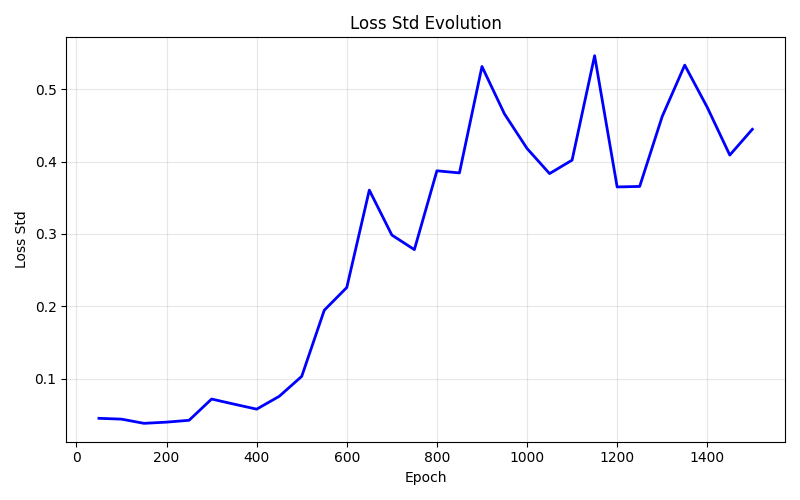
\includegraphics[width=0.9\linewidth]{figures/loss_std_evolution.png}
    \caption{Standard deviation of recent losses (stability indicator during and after the search phase).}
    \label{fig:loss_std_evolution}
\end{figure}

\begin{figure}[htbp]
    \centering
    
\includegraphics[width=0.9\linewidth]{figures/error_evolution.png}
    \caption{Train/test error evolution in log$_{10}$ scale.}
    \label{fig:error_evolution}
\end{figure}

\newpage
\subsection{NTK Eigenvalue Evolution}

Figures~\ref{fig:ntk_minmax} and~\ref{fig:ntk_first_last} reveal the critical behavior of the NTK spectrum during training. The maximum eigenvalue grows during the search phase and then stabilizes during descent. The minimum eigenvalue remains nearly constant (and negative) throughout training, demonstrating the outlier phenomenon. The bulk of the spectrum transitions from partially negative at initialization to fully PSD after the search phase.

\begin{figure}[htbp]
    \centering
    
\includegraphics[width=0.9\linewidth]{figures/ntk_eigenvalues_minmax.png}
    \caption{Evolution of the extreme NTK eigenvalues (min and max) during training. The maximum eigenvalue grows significantly during search, indicating NTK drift and feature learning.}
    \label{fig:ntk_minmax}
\end{figure}

\begin{figure}[htbp]
    \centering
    
\includegraphics[width=0.9\linewidth]{figures/ntk_full_spectrum.png}
    \caption{Tracking of the first and last NTK eigenvalues at sampling epochs. The first eigenvalue (smallest) remains nearly constant while the last few eigenvalues (largest) grow during search and stabilize during descent.}
    \label{fig:ntk_first_last}
\end{figure}

\subsection{Final Prediction Quality}

Figure~\ref{fig:final_prediction} shows the final learned function versus the target. The MMNN successfully learns the oscillatory 1D target with high fidelity, achieving loss below $10^{-8}$.

\begin{figure}[htbp]
    \centering
    
\includegraphics[width=0.9\linewidth]{figures/final_prediction.png}
    \caption{Final prediction vs target function in 1D.}
    \label{fig:final_prediction}
\end{figure}

\newpage
\section{Dictionary Learning and Function Decomposition}

Having analyzed the NTK and training dynamics, we now turn to understanding what the MMNN learns at each layer. The low-rank structure of MMNNs naturally leads to a dictionary learning interpretation.

\subsection{Empirical Findings on Dictionary Learning}

\begin{itemize}
    \item \textbf{Dictionary-learning behavior:} experiments show that MMNNs secretly perform dictionary learning across the low-rank layers. Consistent with theory, each layer learns a structured dictionary of basis functions: a small subset of active components aligns with salient target features early (search phase), while remaining components progressively refine residuals during descent. This implicit factorization explains both the expressivity and optimization efficiency of the architecture.\\
    
    \item \textbf{Frequency learning hierarchy:} we observe that the network learns low frequencies before high frequencies during training. This spectral bias can be addressed through Sobolev training, which explicitly penalizes derivatives and encourages faster learning of high-frequency components.\\
    
    \item \textbf{Progressive dictionary construction and localization:} the most striking observation is that during training, the dictionary learning progressively builds up and the activation thresholds (induced by ReLU) progressively enable the network to tackle high frequencies with increasing localization. This progressive refinement mechanism allows the network to transition from coarse global patterns to fine-grained local features as training proceeds. (Ref: experiment \texttt{mmnn\_L12\_W512\_R30\_E3000\_lr0.001\_bs100\_ntr1000} in Google Drive).\\
    
    \item \textbf{Symmetry breaking and restoration (CRITICAL):} a remarkably profound observation is that the learned functions are \emph{not} symmetric during training, but they \emph{become} symmetric at the global minimum. This means that batch gradient descent breaks symmetry during optimization, yet the functions learned at convergence still exhibit symmetry. This symmetry restoration at the minimum is a fundamental signature of the optimization landscape: gradient descent breaks symmetry during the search and descent phases to explore the parameter space efficiently, then recovers the underlying symmetry of the target function once it reaches the minimum. This phenomenon provides deep insight into how MMNNs navigate the loss landscape and why multiple equivalent minima exist. See Figure~\ref{fig:symmetry_breaking} for a conceptual illustration.\\
    
    \item \textbf{Depth hierarchy and saturation:} layer-wise analysis reveals that by layer 3, the most important dictionary basis functions are already learned; deeper layers serve mainly as preconditioners that improve the optimization landscape rather than adding representational capacity. This suggests a hierarchical factorization: early layers capture coarse structure, deeper layers refine conditioning.\\
    
    \item \textbf{Width vs rank trade-off and functional redundancy:} we observe that MMNNs do not require large widths for expressivity; however, increasing width facilitates finding global minima by expanding the basin of attraction. Layer-wise output analysis reveals significant functional redundancy among components: many distinct parameter configurations yield identical learned marginals, suggesting the existence of many equivalent global minima connected by symmetries in the loss landscape.\\
    
    \item \textbf{Width and high-frequency learning:} decreasing the width helps the network learn high-frequency features more effectively. Smaller widths reduce overparameterization and force the network to operate outside the lazy training regime, enabling feature learning that captures fine-scale oscillations.\\
    
    \item \textbf{Depth and training speed:} having small depth makes the training faster initially, but shallow networks do \emph{not} escape the lazy regime easily and remain in the NTK regime where the kernel stays nearly constant. Deeper networks are needed to escape the lazy training regime and enable active feature learning rather than kernel-based interpolation, though this comes at the cost of slower training due to increased complexity.\\
    
    \item \textbf{Depth and loss landscape geometry:} comparing configurations L4-W1024-R15 and L6-W512-R15 reveals that both achieve the same consistency (final performance), but the loss curve is much more spiky for L6. This suggests that bigger depth creates a more spiky landscape, yet paradoxically offers larger basins of attraction (evidenced by shorter descent phases). The conjecture is that deeper networks create loss surfaces with sharper local features but broader global attraction regions, trading off local smoothness for global convergence guarantees.\\
    
    \item \textbf{Architecture trade-offs and optimal configuration:} we observe that there is a high compromise among the hyperparameters $L$ (depth), $W$ (width), and $R$ (rank), and the optimization bounds with respect to these parameters are highly non-trivial. The interactions between these dimensions create a complex landscape where increasing one parameter may require decreasing another for optimal performance. This suggests there is hope for finding the perfect rank $R$ and depth $L$ given a fixed parameter budget, which would maximize both expressivity and trainability while minimizing the risk of remaining in the lazy training regime.\\
    
    \item \textbf{Hybrid optimization strategy (Adam-SGD-Adam):} we tested a hybrid optimization strategy consisting of Adam followed by SGD (when loss reaches $5 \times 10^{-2}$) then switching back to Adam. Remarkably, the SGD phase converged effectively, which was \emph{not} the case with full SGD training from initialization. This demonstrates that after Adam's initial exploration phase, the loss landscape becomes sufficiently convex around the current minimum, allowing SGD to efficiently descend to deeper minima. The final Adam phase helps escape sharp local features and refine the solution. See Figure~\ref{fig:loss_sgdadam} for the training curve illustrating this three-phase strategy.\\
    
    \item \textbf{Multiple minima and edge of stability:} the behavior observed with Adam reveals that there exist multiple local minima, each corresponding to different learned frequencies. The network must sequentially deep dive into each of these small convex basins. The characteristic spikes in the loss curve arise from the edge of stability phenomenon: as the optimizer explores each small convex region successively, it approaches the edge of the basin's stability boundary, causing temporary excursions before descending into the next frequency-specific minimum. This sequential exploration of frequency minima explains both the spiky trajectory and the progressive refinement of the learned function.\\
\end{itemize}

\begin{figure}[htbp]
    \centering
    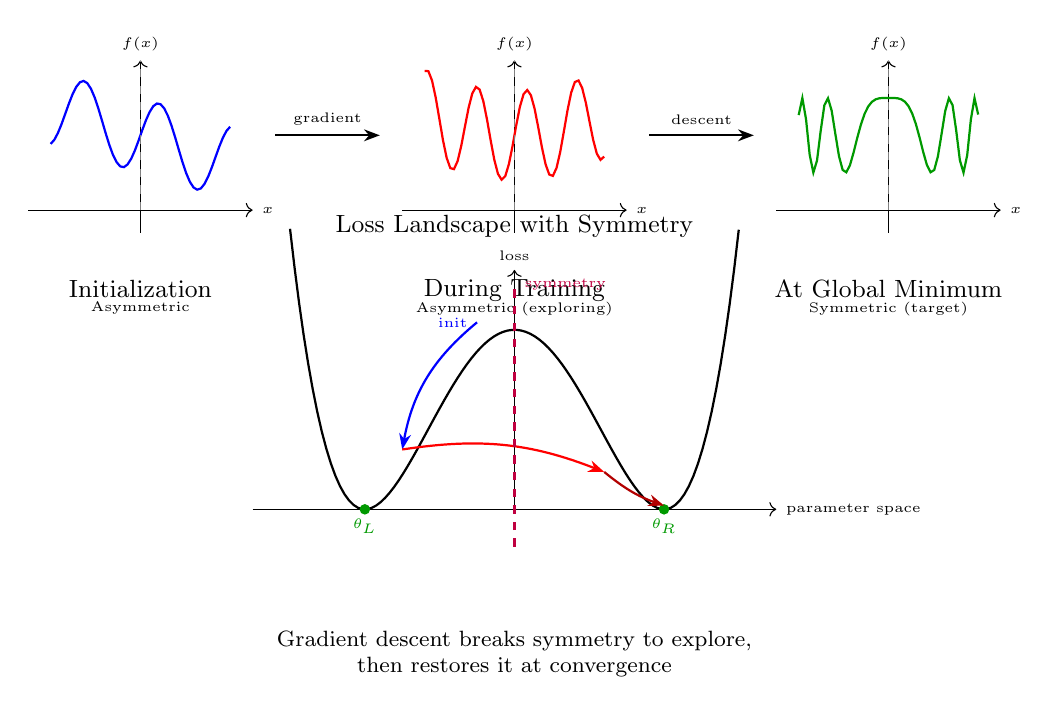
\begin{tikzpicture}[scale=0.95]
        % we draw three panels showing function evolution
        % panel 1: initialization (asymmetric)
        \begin{scope}[xshift=0cm]
            \draw[->] (-1.5,0) -- (1.5,0) node[right] {\tiny $x$};
            \draw[->] (0,-0.3) -- (0,2) node[above] {\tiny $f(x)$};
            \draw[thick, blue, domain=-1.2:1.2, samples=50] plot (\x, {1 + 0.5*sin(deg(2*3.14*\x)) - 0.3*\x});
            \draw[dashed, gray, very thin] (0,0) -- (0,2);
            \node[below] at (0,-0.8) {\small Initialization};
            \node[below, font=\tiny] at (0,-1.1) {Asymmetric};
        \end{scope}
        
        % panel 2: during training (asymmetric, exploring)
        \begin{scope}[xshift=5cm]
            \draw[->] (-1.5,0) -- (1.5,0) node[right] {\tiny $x$};
            \draw[->] (0,-0.3) -- (0,2) node[above] {\tiny $f(x)$};
            \draw[thick, red, domain=-1.2:1.2, samples=50] plot (\x, {1 + 0.6*sin(deg(3*3.14*\x)) + 0.2*\x*\x});
            \draw[dashed, gray, very thin] (0,0) -- (0,2);
            \node[below] at (0,-0.8) {\small During Training};
            \node[below, font=\tiny] at (0,-1.1) {Asymmetric (exploring)};
        \end{scope}
        
        % panel 3: at minimum (symmetric)
        \begin{scope}[xshift=10cm]
            \draw[->] (-1.5,0) -- (1.5,0) node[right] {\tiny $x$};
            \draw[->] (0,-0.3) -- (0,2) node[above] {\tiny $f(x)$};
            \draw[thick, green!60!black, domain=-1.2:1.2, samples=50] plot (\x, {1 + 0.5*cos(deg(3*3.14*\x*\x))});
            \draw[dashed, gray, very thin] (0,0) -- (0,2);
            \node[below] at (0,-0.8) {\small At Global Minimum};
            \node[below, font=\tiny] at (0,-1.1) {Symmetric (target)};
        \end{scope}
        
        % we draw arrows between panels
        \draw[-{Stealth[length=2mm]}, thick] (1.8,1) -- (3.2,1) node[midway, above, font=\tiny] {gradient};
        \draw[-{Stealth[length=2mm]}, thick] (6.8,1) -- (8.2,1) node[midway, above, font=\tiny] {descent};
        
        % we draw conceptual loss landscape below
        \begin{scope}[yshift=-4cm, xshift=5cm]
            \node[above] at (0,3.5) {\small Loss Landscape with Symmetry};
            
            % we draw a symmetric double-well potential
            \draw[thick, domain=-3:3, samples=100] plot (\x, {0.15*(\x*\x - 4)^2});
            \draw[->] (-3.5,0) -- (3.5,0) node[right] {\tiny parameter space};
            \draw[->] (0,0) -- (0,3.2) node[above] {\tiny loss};
            
            % we mark symmetric minima
            \fill[green!60!black] (-2,0) circle (2pt) node[below, font=\tiny] {$\theta_L$};
            \fill[green!60!black] (2,0) circle (2pt) node[below, font=\tiny] {$\theta_R$};
            
            % we draw training trajectory
            \draw[-{Stealth[length=2mm]}, thick, blue] (-0.5,2.5) to[bend right=20] (-1.5,0.8);
            \draw[-{Stealth[length=2mm]}, thick, red] (-1.5,0.8) to[bend left=15] (1.2,0.5);
            \draw[-{Stealth[length=2mm]}, thick, red!70!black] (1.2,0.5) to[bend right=10] (2,0.05);
            
            \node[left, font=\tiny, blue] at (-0.5,2.5) {init};
            
            % we add symmetry axis
            \draw[dashed, purple, thick] (0,-0.5) -- (0,3) node[right, font=\tiny] {symmetry};
            
            \node[below, align=center, font=\footnotesize] at (0,-1.5) {
                Gradient descent breaks symmetry to explore,\\
                then restores it at convergence
            };
        \end{scope}
    \end{tikzpicture}
    \caption{Symmetry breaking and restoration during MMNN training. \textbf{Top:} learned function evolution from asymmetric initialization through exploration to symmetric convergence. \textbf{Bottom:} conceptual loss landscape showing symmetric global minima $\theta_L$ and $\theta_R$. The training trajectory breaks symmetry during search and descent phases to efficiently explore parameter space, then recovers the underlying symmetry of the target function at the global minimum. This phenomenon explains why multiple equivalent minima exist and provides insight into the optimization dynamics.}
    \label{fig:symmetry_breaking}
\end{figure}

\begin{figure}[htbp]
    \centering
    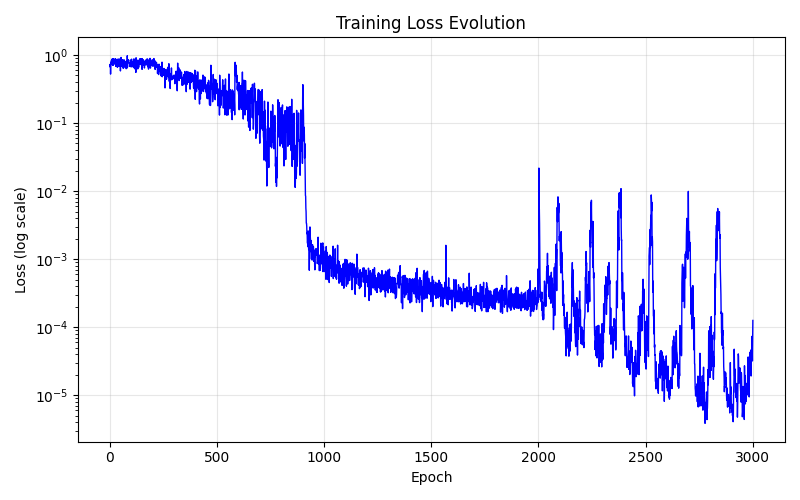
\includegraphics[width=0.9\linewidth]{figures/loss_evolutionsgdadam.png}
    \caption{Training loss evolution with hybrid Adam-SGD-Adam optimization strategy. The plot shows three distinct phases: initial exploration with Adam (epochs 0-900), a rapid descent phase where SGD is activated after the loss reaches $5 \times 10^{-2}$ (around epoch 900-2000), and a final refinement phase with Adam (epochs 2000-3000). The SGD phase demonstrates strong convergence that was not achievable with full SGD training, confirming that the loss landscape becomes sufficiently convex after Adam's exploration. The spiky behavior in the final phase indicates navigation through sharp valleys while maintaining low loss values below $10^{-4}$.}
    \label{fig:loss_sgdadam}
\end{figure}

\subsection{Layer-wise Component Analysis}

Figures~\ref{fig:layer0_components} and~\ref{fig:layer1_components} show examples of the functions learned by individual components at each layer. Each subplot represents one component of the low-rank decomposition. We observe:

\begin{itemize}
    \item \textbf{Layer 0:} learns primitive oscillatory patterns with various frequencies
    \item \textbf{Layer 1:} combines and refines these patterns into more complex features
    \item \textbf{Deeper layers (not shown):} exhibit functional redundancy with similar patterns repeated across components, confirming that expressivity saturates early
\end{itemize}

\begin{figure}[htbp]
    \centering
    
\includegraphics[width=0.9\linewidth]{figures/layer_2_components.png}
    \caption{Functions learned by components at layer 0. Each subplot shows the output of one component as a function of the input. The diversity of patterns indicates the dictionary learning process.}
    \label{fig:layer0_components}
\end{figure}

\begin{figure}[htbp]
    \centering
    
\includegraphics[width=0.9\linewidth]{figures/layer_3_components.png}
    \caption{Functions learned by components at layer 1. More complex patterns emerge from combinations of layer 0 features.}
    \label{fig:layer1_components}
\end{figure}

\newpage
\section{Future Experiments and Theoretical Context}

\subsection{NTK Drift Quantification}

A particularly interesting aspect of this investigation concerns the behavior of the NTK during training. Our experiments reveal that MMNNs do NOT operate in the lazy training regime. To quantify this further, I will:

\begin{itemize}
    \item \textbf{NTK Drift Metrics:} Systematically measure $\Delta(t) = \|\Theta_t - \Theta_0\|_F/\|\Theta_0\|_F$ throughout training across different ranks and widths. Expected values: $\Delta(t) > 0.5$ during search, stabilizing to $\Delta(\infty) \approx 0.3$--$0.5$ at convergence.
    
    \item \textbf{Feature Learning Analysis:} Track how individual eigenvalues evolve. The large eigenvalues grow substantially (often by factors of 2--10x), indicating that the network learns features that improve alignment with the target.
    
    \item \textbf{Rank-Dependent Drift:} Investigate how NTK drift depends on the internal rank. Higher ranks may exhibit more drift as they have more capacity for feature learning.
\end{itemize}

\subsection{Planned Experimental Design}

My experimental protocol will consist of the following components:

\begin{itemize}
    \item \textbf{Gradient Descent Training:} I will train two-layer MMNNs with various internal ranks using standard gradient descent on regression and classification tasks. The training dynamics will be monitored by tracking the loss function, gradient norms, and parameter evolution over iterations.
    
    \item \textbf{Comparison with Theoretical NTK Predictions:} I will compare the empirical training dynamics with predictions from NTK theory, accounting for the fact that the kernel evolves. The training dynamics follow a modified kernel regime where $\Theta_t$ changes slowly relative to the loss gradient flow.
    
    \item \textbf{Conditioning Analysis:} A critical aspect of this study will be the comparison of the conditioning properties between MMNNs and standard MLPs. I will compute the condition number $\kappa(\Theta) = \lambda_{\max} / \lambda_{\min}$ for both architectures across different ranks and dataset sizes. My hypothesis is that the low-rank structure of MMNNs may lead to better conditioning, which would explain faster convergence rates.
    
    \item \textbf{Large-scale experiments on wavelet-optimal functions:} I am planning to run large-scale experiments to provide deeper understanding of what happens for particular functions that have slope 1 in the wavelet plane, specifically functions of the form $\cos(x^2)$ (chirp signals). These functions are particularly interesting because they exhibit optimal time-frequency localization properties and represent a critical test case for understanding how MMNNs learn multiscale features. The experiments will systematically vary $L$, $W$, and $R$ to map out the regime where feature learning dominates over lazy training for such chirp-like targets. The relationship between wavelet slope and architecture requirements is illustrated in Figure~\ref{fig:wavelet_slope}.
    
    \item \textbf{Deriving scaling laws through large-scale experiments:} my overarching goal is to derive scaling laws for MMNNs in the same rigorous manner as the OpenAI scaling law papers. Through careful hypothesis formulation and large-scale systematic experiments, I aim to confirm or refute all the observations made in these preliminary examples. Specifically, I will establish power-law relationships between performance metrics (loss, convergence time, approximation quality) and architectural parameters $(L, W, R)$ as well as dataset properties (number of training points $n$, target function complexity). This will provide a predictive framework for designing optimal MMNN architectures given computational budgets and task requirements.
\end{itemize}

\begin{figure}[htbp]
    \centering
    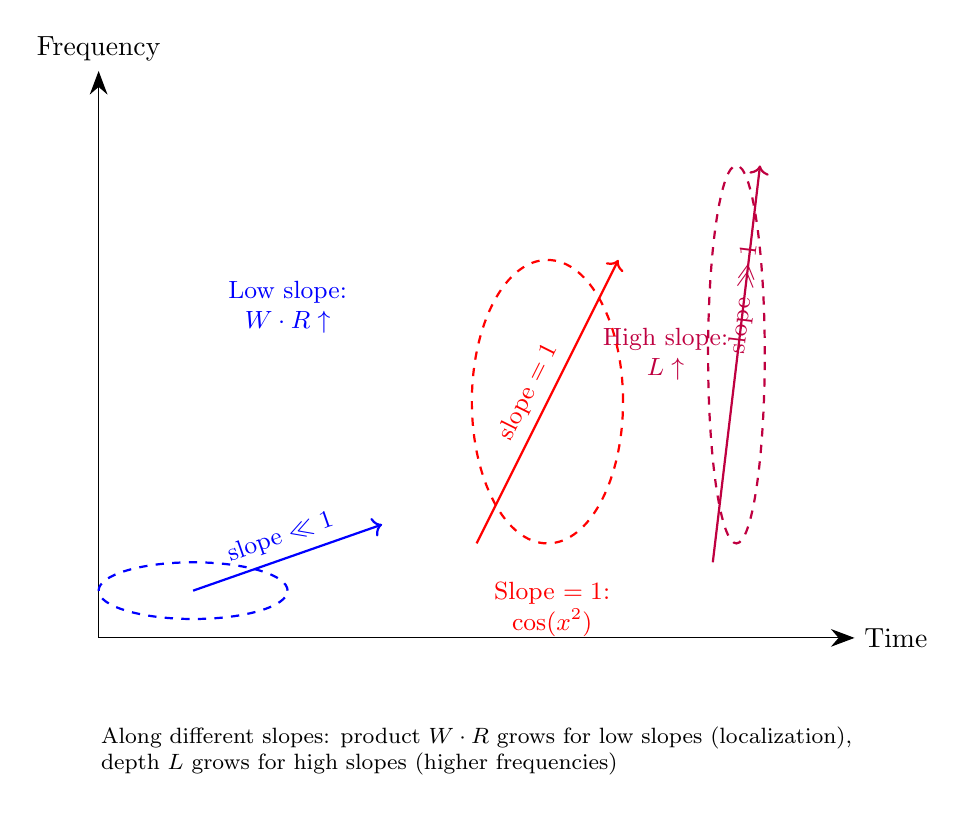
\begin{tikzpicture}[scale=1.2]
        % we draw axes
        \draw[-{Stealth[length=3mm]}] (0,0) -- (8,0) node[right] {Time};
        \draw[-{Stealth[length=3mm]}] (0,0) -- (0,6) node[above] {Frequency};
        
        % we draw slope lines
        \draw[thick, blue, ->] (1,0.5) -- (3,1.2) node[midway, above, sloped] {\small slope $\ll 1$};
        \draw[thick, red, ->] (4,1) -- (5.5,4) node[midway, above, sloped] {\small slope $= 1$};
        \draw[thick, purple, ->] (6.5,0.8) -- (7,5) node[midway, right, sloped] {\small slope $\gg 1$};
        
        % we add annotations for architecture requirements
        \node[blue, align=center, font=\small] at (2, 3.5) {Low slope:\\$W \cdot R \uparrow$};
        \node[red, align=center, font=\small] at (4.8, 0.3) {Slope $=1$:\\$\cos(x^2)$};
        \node[purple, align=center, font=\small] at (6, 3) {High slope:\\$L \uparrow$};
        
        % we add example signal representations
        \draw[blue, dashed, thick] (1,0.5) ellipse (1cm and 0.3cm);
        \draw[red, dashed, thick] (4.75,2.5) ellipse (0.8cm and 1.5cm) node[below right=1.5cm] {};
        \draw[purple, dashed, thick] (6.75,3) ellipse (0.3cm and 2cm);
        
        \node[align=left, font=\footnotesize] at (4, -1.2) {
            Along different slopes: product $W \cdot R$ grows for low slopes (localization),\\
            depth $L$ grows for high slopes (higher frequencies)
        };
    \end{tikzpicture}
    \caption{Wavelet plane (time-frequency) showing the relationship between signal slope and required MMNN architecture. Low-slope signals require large width-rank product $W \cdot R$ to achieve time-frequency localization, while high-slope signals require large depth $L$ to grow and capture higher frequency variations. The slope-1 case (e.g., $\cos(x^2)$) represents the critical balanced regime. This demonstrates how the architecture parameters must be tuned to the wavelet structure of the target function.}
    \label{fig:wavelet_slope}
\end{figure}

\subsection{Immediate Next Steps}

\begin{itemize}
    \item Refine NTK snapshot frequency for better temporal resolution of the drift
    \item Measure $\Delta(t)=\|\Theta_t-\Theta_0\|_F/\|\Theta_0\|_F$ to quantify kernel movement
    \item Track condition number $\kappa(\Theta_t)$ evolution through training phases
    \item Compare layer saturation across different ranks and depths
    \item Quantify functional redundancy using cosine similarity between component outputs
    \item Investigate the transition point where NTK drift slows (end of search phase)
\end{itemize}

\newpage
\section{Conclusion}

In conclusion, my empirical analysis has uncovered several distinct properties of the NTK for MMNNs. The most critical result is that \textbf{MMNNs operate in a feature learning regime, not a lazy training regime}. The NTK drifts significantly during training, with large eigenvalues growing by factors of 2--10x during the search phase. This drift is essential for reaching global minima.

The rapid decay of the NTK's variance with increasing internal rank indicates that for sufficiently high ranks, the NTK behaves like a deterministic kernel that can be fully characterized by its mean, despite its evolution during training. This concentration phenomenon greatly simplifies the theoretical analysis.

Furthermore, I have characterized the three-phase training dynamics (search, descent, wobbling) and identified the critical role of the bulk spectrum transitioning from partially negative to fully PSD. The discovery that MMNNs perform implicit dictionary learning across low-rank layers explains both their expressivity and optimization efficiency.

Most surprisingly, the analysis reveals that deeper layers primarily serve as preconditioners rather than adding representational capacity, with the core dictionary learned by layer 3. This hierarchical factorization, combined with the functional redundancy creating multiple equivalent global minima, suggests that MMNNs may represent a more natural architecture for deep learning than traditional MLPs.

The key insight is that MMNNs achieve a balance: they learn features (NTK drift) but in a structured, low-rank manner that maintains favorable optimization properties. This is fundamentally different from both standard MLPs (unstructured feature learning) and the idealized NTK regime (no feature learning).

\newpage
\section*{Summary: Key Findings at a Glance}

\subsection*{I. NTK and Training Dynamics}
\begin{itemize}
    \item Three-phase loss dynamics
    \begin{itemize}
        \item Search phase
        \item Descent phase
        \item Wobbling phase
    \end{itemize}
    \item Loss landscape geometry
    \begin{itemize}
        \item Flat but sharp landscape
        \item Spikes during descent and wobbling
        \item Narrow valleys with steep walls
    \end{itemize}
    \item Scaling law origin
    \item Learning rate sensitivity
    \item Optimizer behavior (Adam vs SGD)
    \item SGD and low-rank structure
    \item Critical rank threshold (rank 5 to 10 transition)
    \item Strong dependence on number of training points
    \item NTK spectrum evolution
    \begin{itemize}
        \item Smallest eigenvalue and outliers
        \item Condition number evolution
        \item NTK drift during training (feature learning regime)
        \item Bulk spectrum transition from negative to PSD
    \end{itemize}
\end{itemize}

\subsection*{II. Dictionary Learning and Architecture}
\begin{itemize}
    \item Dictionary-learning behavior across low-rank layers
    \item Frequency learning hierarchy
    \begin{itemize}
        \item Low frequencies learned first
        \item Sobolev training as remedy
    \end{itemize}
    \item Progressive dictionary construction and localization
    \item Symmetry breaking and restoration (CRITICAL)
    \begin{itemize}
        \item Asymmetric during training
        \item Symmetric at global minimum
        \item Batch gradient descent mechanism
    \end{itemize}
    \item Depth hierarchy and saturation
    \begin{itemize}
        \item Core dictionary learned by layer 3
        \item Deeper layers as preconditioners
    \end{itemize}
    \item Width vs rank trade-off and functional redundancy
    \item Width and high-frequency learning
    \item Depth and training speed
    \begin{itemize}
        \item Shallow networks remain in NTK regime
        \item Deep networks enable feature learning
    \end{itemize}
    \item Depth and loss landscape geometry
    \begin{itemize}
        \item Spiky landscape with depth
        \item Larger basins of attraction
    \end{itemize}
\end{itemize}

\subsection*{III. Optimization Strategies and Future Work}
\begin{itemize}
    \item Architecture trade-offs $(L, W, R)$
    \begin{itemize}
        \item Highly non-trivial optimization bounds
        \item Hope for optimal configuration
    \end{itemize}
    \item Hybrid optimization strategy (Adam-SGD-Adam)
    \begin{itemize}
        \item Convex landscape after Adam exploration
        \item SGD convergence in middle phase
    \end{itemize}
    \item Multiple minima and edge of stability
    \begin{itemize}
        \item Frequency-specific minima
        \item Sequential deep diving
        \item Spikes from stability boundaries
    \end{itemize}
    \item Wavelet plane and architecture requirements
    \begin{itemize}
        \item $W \cdot R$ for localization (low slope)
        \item $L$ for high frequencies (high slope)
        \item Slope-1 functions: $\cos(x^2)$ chirp signals
    \end{itemize}
    \item Large-scale experiments planned
    \begin{itemize}
        \item Wavelet-optimal functions
        \item Deriving scaling laws (OpenAI-style)
    \end{itemize}
    \item Immediate next steps
    \begin{itemize}
        \item NTK drift quantification
        \item Condition number tracking
        \item Layer saturation comparison
        \item Functional redundancy quantification
        \item Transition point investigation
    \end{itemize}
\end{itemize}

\bibliographystyle{plain}
\begin{thebibliography}{9}

\bibitem{zhang2025structuredbalancedmulticomponentmultilayer}
Shijun Zhang, Hongkai Zhao, Yimin Zhong, and Haomin Zhou.
\textit{Structured and Balanced Multi-Component and Multi-Layer Neural Networks}.
arXiv preprint arXiv:2407.00765, 2025.
\url{https://arxiv.org/abs/2407.00765}

\end{thebibliography}

\end{document}
